\section{Other Related Works}

% \textbf{Characterizing Effective CoT} \citet{gandhi2025cognitive} identify four cognitive behaviors, including verification and backtracking, that correlates with reasoning performance on model level. 

\citet{golovnevaroscoe} propose a suite of metrics for step-by-step reasoning (e.g., alignment, hallucination, commonsense), computed from sentence-level embeddings. Their analysis targets models producing relatively short CoTs; extending these embedding-based metrics to modern LRMs that generate very long CoTs (tens to hundreds of thousands of tokens) is nontrivial and computationally burdensome. Consequently, it is unclear how to apply that framework in our setting.

Related to \length, the efficiency of CoT reasoning \citep{zhang2025reasoning, an2025don, gao2025far} is another desirable property since we prefer correct solutions achieved with minimal computation. However, efficiency is only well defined for \emph{correct} CoTs and is ambiguous for incorrect ones; accordingly, we do not analyze efficiency in this paper and focus instead on metrics applicable to both correct and incorrect traces.




\section{Details on the Generations}

\subsection{Models and Prompts}

We leverage all these models:

\textit{Proprietary models with CoT access}:  Claude 3.7 Sonnet Thinking \citep{anthropic2025claude37}, Grok 3 mini \citep{xai2025grok3mini},

\textit{Open Sourced Families}: Deepseek R1 (0120), Deepseek Distill Qwen 32B (Deepseek 32B), Deepseek Distill Qwen 7B (Deepseek 7B), Qwen 3 235B \citep{yang2025qwen3}, Qwen 3 32B, Qwen 3 8B, GPT oss 120B \citep{agarwal2025gptoss}, GPT oss 20B.


For all the reasoning models, we generate 16 response with 4 temperature, 0.3, 0.6, 0.8, and 1.0. The top p is always set to be 0.9. Claude 3.7 Thinking only allows generation with temperature 1.0, so we use 1.0 for all the generation. For GPT oss 120B and GPT oss 20B, we use the medium thinking mode.

The prompt used for AIME and HARP is:

\fbox{\parbox{0.9\textwidth}{
Solve the following math problem efficiently and clearly. Please reason step by step, and put your final answer within \$\textbackslash boxed\{answer\}\$.\\
Where [answer] is just the final number or expression that solves the problem.\\
Problem: \{Question\}
}}

The prompt used for GPQA-Diamond is:

\fbox{\parbox{0.9\textwidth}{
What is the correct answer to this question: \\
\{Question\} \\
\{Choices\} \\
Format your response as follows: "The correct answer is (insert answer here)".
}}

In the experiment of continuation generation, we follow the suggested optimal temperature 0.6 for all models. For test-time selection, we generate 64 CoTs similarly, using four temperatures with 16 CoTs per temperature.

Across all evaluations, we define the CoT as the text between \texttt{<think>} and \texttt{</think>} (or the model-specific equivalents) for all ten models. All annotations and evaluations are performed exclusively on this thinking portion.

\subsection{Evaluation}

We use the Math-verify package \citep{Math-Verify} to evaluate the correctness for math reasoning.

For GPQA-Diamond, we parse outputs using the answer template. Because some smaller models do not consistently follow the required format in the prompt, we augment the parser with additional templates to robustly extract the final answer, ensuring correlations are computed against true answer correctness.

\subsection{Keywords for Chunking}

We report the full list of keywords used for chunking in Table \ref{app-tab1:keywords}.

\begin{table}[h]
\centering
\begin{tabular}{@{}p{4cm}p{4cm}p{4cm}@{}}
\toprule
\multicolumn{3}{c}{\textbf{Keywords}} \\
\midrule
Wait & Let me step back & Hang on \\
Hold on & Let me double check & Hold on a minute \\
Hold on a second & Am I missing something & Alternatively \\
Instead & Similarly & I'll approach this from another angle \\
Let's explore alternative approaches & Looking at other approaches & Let me check \\
But let's check & But wait & Let's check \\
I should check & Let me verify & Let's verify \\
Another thought & I should double-check & Let me double-check \\
Let me re-examine & Let me confirm & Looking at the options \\
Looking at the answer choices & Let's look at the options & Let's look at each choice \\
Looking at the other choices & Looking at the answer options & Let me just confirm \\
Another angle & Another check & Let's think again \\
Let's also think about & Let me think about & Another point \\
So back to & Another possibility & Let's proceed step by step\\
Looking at the candidate answers & second thought & Let’s break it down \\
Let me reconsider & Let's go back & re-analyze \\
re-check & reconsider & re-examine \\
First, & go though each option & another approach \\
\bottomrule
\end{tabular}
\caption{Collection of Keywords}
\label{app-tab1:keywords}
\end{table}

\section{Loxical Metrics}\label{appendix:loxical}

We first assess the quality of the \Review annotations by comparing them with human labels. We then describe the motivation-annotation pipeline in Appendix~\ref{append-motivation}. Finally, we report the generalized linear mixed-effects model (GLMM) specification and results in Appendix~\ref{append:glmm}.


% \subsection{Review Annotation}

% Here is the prompt for asking Maverick model to annotate \texttt{Progress} and \Review. We use temperature 0.3 for the annotation.

% \fbox{\parbox{0.9\textwidth}{
% Classify this chunk using the following categories: [progress, review].

% Here is the definition:

% Review: A step that reads, checks, restates, deletes, or rewinds existing material without pushing the frontier forward. This includes:

% - Verification: read-only checks, cross-tests, rereading the prompt, expressions of doubt that leave prior work untouched;

% - Verification using alternative methods or calculations that confirm previous conclusions (even if they involve new work), including recalculations, double-checking, or exploring alternative approaches to reach the same conclusion

% - Testing with examples or edge cases to validate existing reasoning.

% - Backtracking: any deletion, overwrite, or "jump back" that abandons a branch before writing the correction

% - Error identification and correction that examines previously stated work.

% - Sections that begin with verification language that primarily serve to verify rather than advance, even if they contain new calculations

% - Checking the question statement for whether choices exist is review.

% - When the outcome result is already reached, further chunks should be classfied as review. The exception is for multi-choice question, when the model checks other options.

% Progress: A step that extends the active reasoning frontier, producing information the solver will rely on later. This includes:

% - Typical signals: new equation, new inference, first-time evaluation of an option, final answer line.

% - For multi-choice questions, the first time evaluating an option is progress, even if the option is incorrect.

% - New reasoning contribute towards solving the problem is progress.

% - Initial problem understanding and knowledge establishment counts as progress, even if expressed with uncertainty.
% }}

\subsection{Alignment with Human Annotations}\label{appendix:alignment_review}

Recall that we leverage the Maverick model to label each chunk into \progress or \review, with the following definition:

\begin{description}
\item \textit{progress}: advances the active reasoning frontier, producing information that later steps rely on.
\item \textit{review}: reads, checks, restates, deletes, or rewinds existing material without advancing the frontier.
\end{description}

We study how reliable the model’s annotation is when acting as a judge—a consideration often missing from LLM-as-judge work. To evaluate this, we collect 30 long reasoning traces from Deepseek R1 and Qwen 3 235B, spanning math and general science, in both free-form and multiple-choice settings. Each trace is segmented into chunks (around 40 per trace on average), and each chunk is labeled by the authors as \progress or \review. We then compare these human labels to the model’s own annotations.

In this way,  we obtain the confusion matrix shown in Table \ref{tab:review_confusion}, which illustrates the accuracy of the annotation at the character level. When considering \review as the positive class, the pipeline demonstrates a low type I error, meaning it rarely misclassifies \progress as \review. We allow the model to misclassify some \review as \progress, as this serves as a lower bound for \review.

\begin{table}[h]
\centering
\begin{tabular}{l|c|c}
\textbf{True\textbackslash Predicted} & \review & \progress \\
\hline
\review & 53.8\% & 10.2\% \\
\progress & 1.2\% & 34.8\% \\
\end{tabular}
\caption{Confusion Matrix for \progress and \review annotation.}
\label{tab:review_confusion}
\end{table}

\subsection{Motivation Annotation}\label{append-motivation}

Besides \review, we hypothesize, drawing on insights from cognitive science \citep{facione1990critical}, that \texttt{Motivation} is a key feature: whether the model exhibits a clear goal and strong motivation behind each action, especially during reviews. Accordingly, we measure the motivation level for all review chunks labeled in the previous section.

We use the same chunking protocol. For each review chunk, with its preceding 5 and following 5 chunks as context, we ask the model to annotate the current chunk’s motivation as \texttt{clear}, \texttt{semiclear}, or \texttt{unclear}. Definitions:

\begin{description}
    \item[] \textit{Clear motivation}: The chunk states a review action (verify / re-check / backtrack / reread…) and cites a specific trigger / rationale for that action, such as a rule number, mismatch, explicit ambiguity, or other concrete evidence.
    \item[] \textit{Semi-Clear motivation}: The chunk states a review action and gives only a generic reason (“make sure it’s correct”, “something seems off”, “to be safe”) with no concrete trigger.
    \item[] \textit{Unclear motivation}: The chunk shows a review action but gives no stated rationale at all; the motive must not be inferred.
\end{description}

The motivation score is computed at the character level: for each character within \Review spans, we assign 1.0 for clear motivation, 0.5 for semi-clear, and 0.0 for unclear, then average over all \Review characters. We defer the correlation results of \texttt{Motivation} to Appendix \ref{append:other metrics}. 

\subsection{Correlation with GLMM}\label{append:glmm}

Apart from the conditional correlation test, we also leverage a Generalized Linear Mixed Model (GLMM) to learn the correlations. For a metric $m$, GLMM fits the following equation to estimate the effect of $m$ on accuracy:
\begin{description}
    \item[\textbf{GLMM model:}] 
    \begin{equation}\label{eqn:glmm}
\text{logit}(P(acc_i)) = \beta_0 + \beta_1 m_i + u({\text{question}_i}).
\end{equation}
\end{description}

The GLMM addresses question-level heterogeneity via a question-specific random intercept \(u_{\text{question}(i)}\) with a Gaussian prior. Here, \(i\) indexes reasoning traces, and \(\operatorname{logit}\) denotes the logistic link function. We interpret \(\beta_1\) as the association (direction and magnitude) between the metric and correctness. The Gaussian prior enables estimating the posterior mean and standard deviation of \(\beta_1\). Thus we also derive Wald-style \(p\)-values to assess significance.

We summarize the GLMM results in Figure~\ref{fig:correlation_all_glmm}. Compared with Figure~\ref{fig:correlation_harp_all_3}, the pattern of colored cells largely matches: whenever the conditional-correlation analysis flags a significant effect, the GLMM yields a coefficient with the same sign and significance. This concordance provides a second line of evidence supporting our findings.

\begin{figure}[tb]
    \centering
    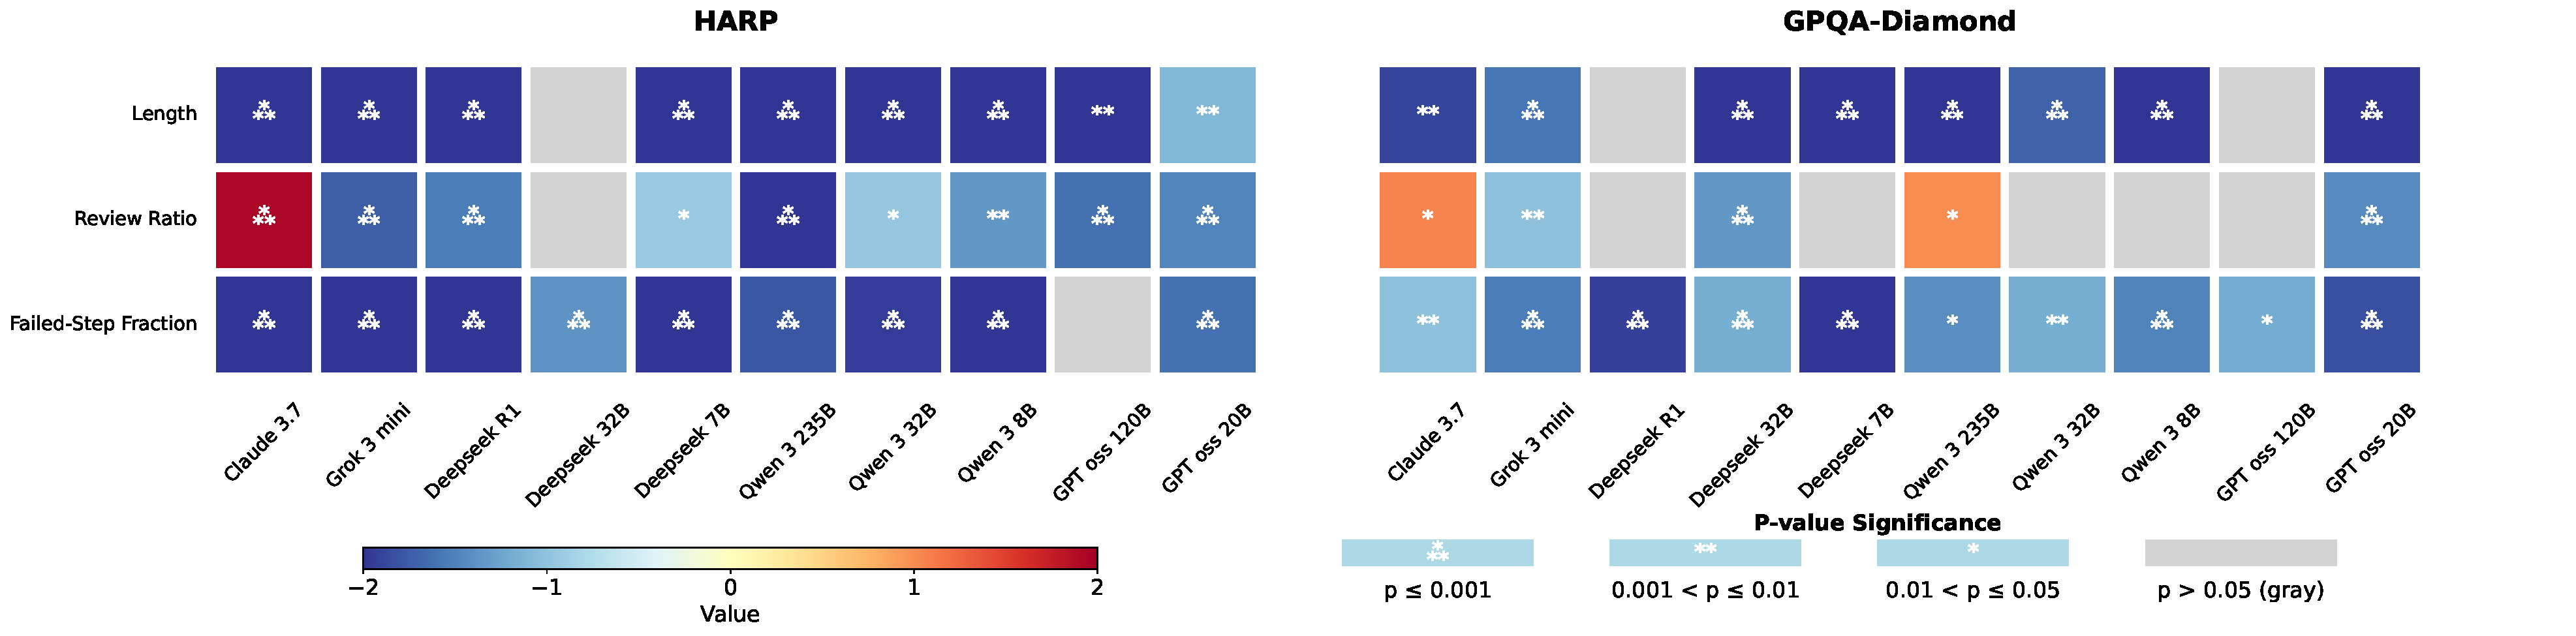
\includegraphics[width=1.05\linewidth]{final_figs/correlation_all_glmm.pdf}
    \caption{GLMM coefficients estimated on the full dataset. Coefficients are shown with a color scale; non-significant cells (\(p>0.05\)) are grayed out, and * denotes statistical significance. More colored cells indicate broader prevalence of correlation; darker colors denote stronger correlations. We observe strong alignment with the conditional-correlation patterns shown in Figure~\ref{fig:correlation_harp_all_3}. This concordance provides a second line of evidence.}
    \label{fig:correlation_all_glmm}
\end{figure}

\subsection{Other Metrics}\label{append:other metrics}

We also evaluate correlations between accuracy and the following metrics:
\begin{itemize}
    \item \texttt{Review Centroid}: the median position of all \review\ chunks within a trace, normalized to $[0,1]$.
    \item \texttt{Review Chunk Fraction}: the fraction of chunks labeled \review\ among all chunks.
    \item \texttt{Review$\rightarrow$Progress Switch Count}: the number of transitions where a \review\ chunk is followed by a \progress\ chunk, normalized by the total number of chunks.
    \item \texttt{Motivation Score}: the fraction of \review\ chunks that state a clear motivation for the action (details in Appendix~\ref{append-motivation}).
    \item \texttt{First Failed-Step Depth}: the depth of the first failed step in the reasoning graph.
    \item \texttt{Reasoning Depth}: the depth of the reasoning graph from the problem statement.
\end{itemize}

\paragraph{Results.}
Figure~\ref{fig:motivation_all_correlation} reports the correlations. Many effects are not consistent across models, for example, the position of \Review\ often behaves like a model-specific stylistic feature rather than a general predictor. Nonetheless, we observe the following patterns:
(i) Correlations are stronger and more frequent in math reasoning than in general scientific reasoning;
(ii) \texttt{Review-Chunk Fraction} shows weaker and more unstable association with accuracy, compared with \fsf, suggesting that graph-level metrics are the more informative granularity;
(iii) \texttt{Motivation Score} exhibits mixed, model-dependent correlations. This feature is intuitively important for human reasoning, as it gauges whether each action is taken with a clear purpose. For LRMs, however, it shows no consistent correlation with accuracy, suggesting their reasoning dynamics can differ from human patterns. (iv) For math reasoning, nearly all models show a positive association between \texttt{Reasoning Depth} and accuracy.

In addition to these metrics, we report analyses of other graph-based measures as well as entropy and progressiveness; see Appendices~\ref{appendix:graph} and \ref{append:further}. A model-level correlation analysis in Appendix~\ref{append:further} shows that models exhibit different generation styles, so comparing metrics \emph{across} models may be biased. This supports our methodology: estimate correlations \emph{within} each model, then seek patterns that replicate \emph{across} models.



% \todo{Create a distributional graph for length, review ratio, for math and GPQA}

% \todo{plot the distribution of failed steps across different models. Do better model good at having more backtracking?}

% \todo{We could also talk about how different model differ in these metrics; Does model A has more accuracy by having metric B higher than Model C?}

\begin{figure}[tb]
    \centering
    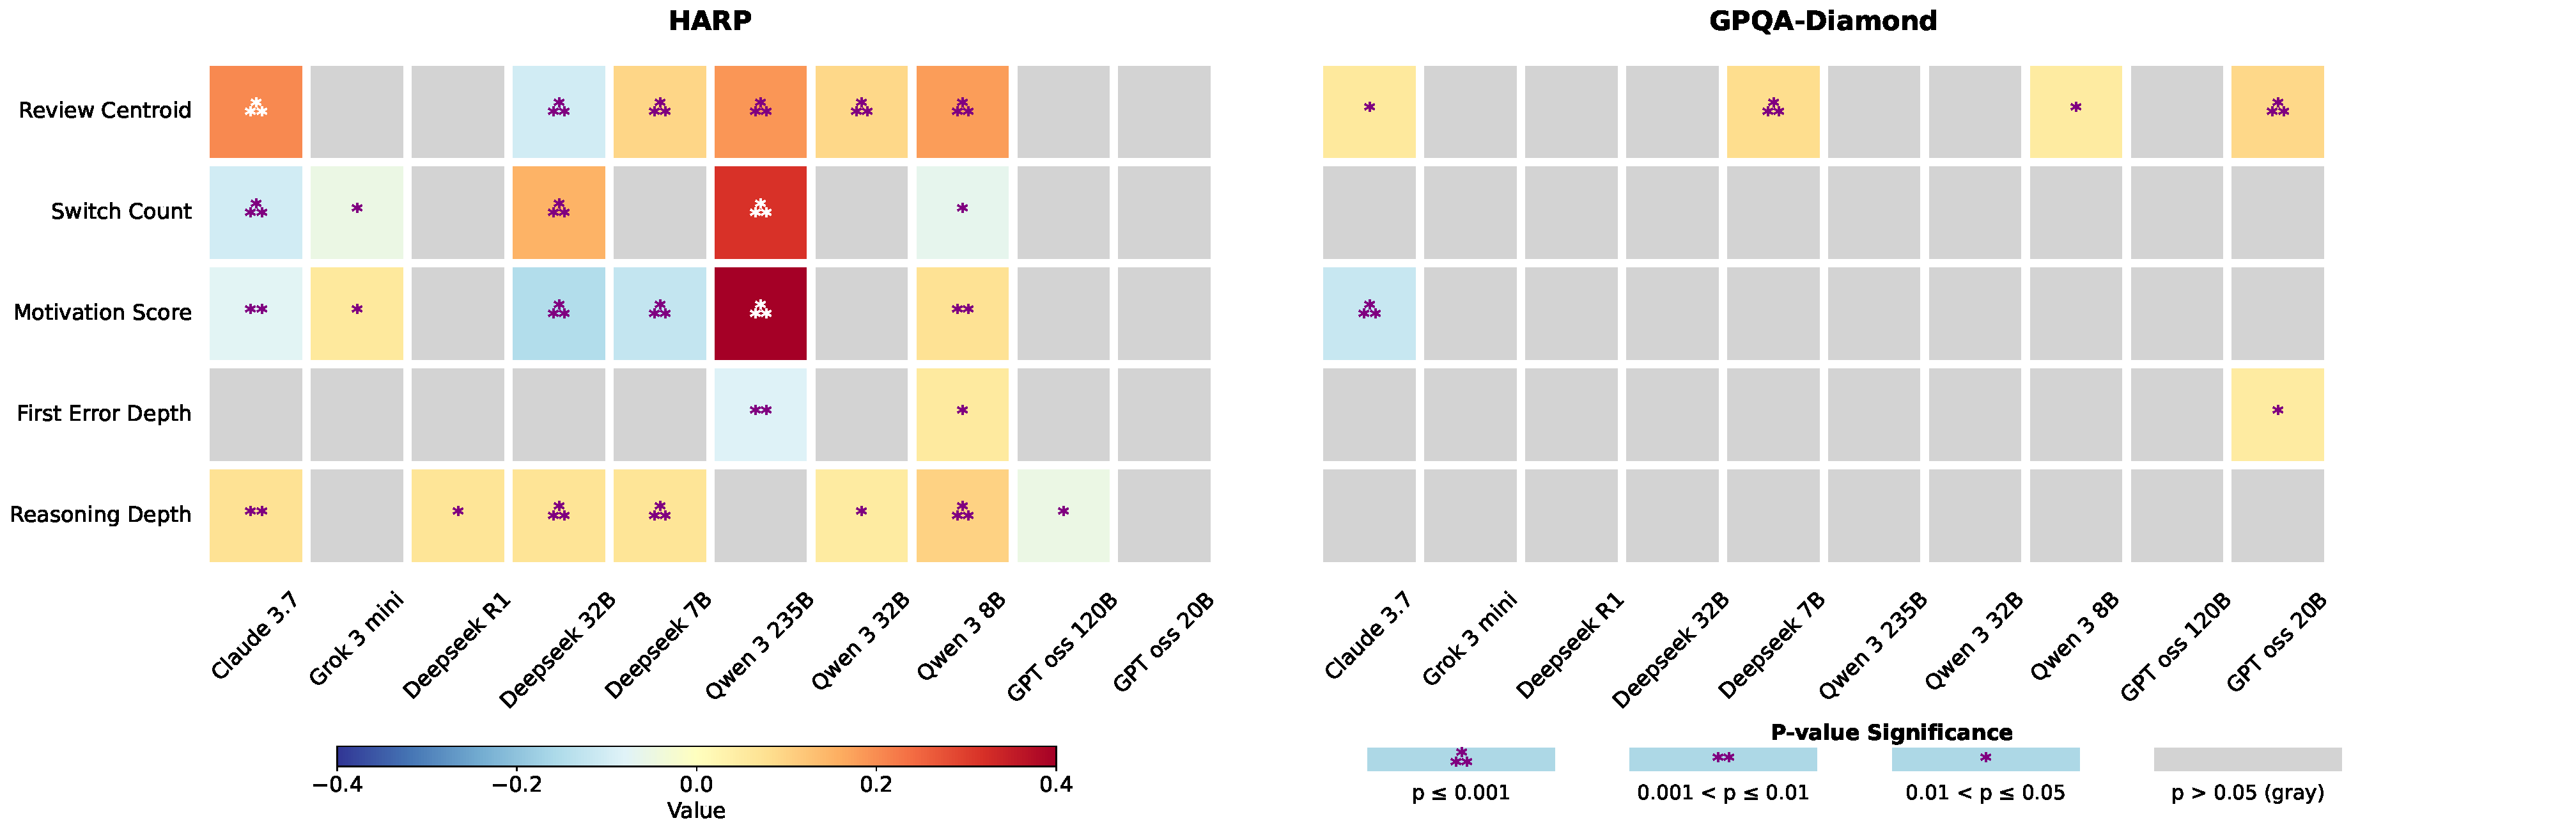
\includegraphics[width=1.08\linewidth]{final_figs/correlation_motivation.pdf}
    \caption{Conditional correlations computed on the full dataset, for \Review position, \texttt{Motivation Score}, \texttt{First Failed-Step Depth}, and overall \texttt{Reasoning Depth}. Again, correlations are shown with a color scale; non-significant cells (\(p>0.05\)) are grayed out, and * denotes statistical significance (see the legend). We color * white or purple for visualization only. }
    \label{fig:motivation_all_correlation}
\end{figure}

\section{Graph Metrics}\label{appendix:graph}

The prompt for generating the reasoning graph:

\fbox{\parbox{0.9\textwidth}{
Parse the reasoning trace into a Graphviz diagram. Focus on these essentials:
\\
\\
Node Rules:

- One node per distinct reasoning step

- `fillcolor=lightblue': Successful reasoning steps

- `fillcolor=lightpink': Failed attempts
\\
\\
Edge Rules:

- Connect node A $\rightarrow$ node B if the information or insight from A is actually used to construct the reasoning in B; branch new attempts from their starting ancestor, not from dead ends.
\\
\\
Requirements:

- Use `rankdir=TB'

- Include ALL attempts (including failures), do not miss any steps in the reasoning.

- ALWAYS start with a "problem statement" node

- ALWAYS end with a "final answer" node 

- Do NOT reorder or reorganize the reasoning flow
\\
\\
Generate complete Graphviz DOT code in dot blocks.
}}

% \todo{Add more visualization for comparison between annotation and graphs.}

\subsection{Extra Graphical Metrics}

A complete list of features we extract from the reasoning graph:

\textbf{Failed steps features}

\texttt{Failed-Step Fraction}: Proportion of nodes marked as failed steps, indicating the density of failed attempts in the reasoning process.

\texttt{Recovery Efficiency}: Average distance from failed nodes to successful nodes, measuring how quickly failed attempts can be corrected.

\textbf{Logical Flow Features}

\texttt{Branching Quality}: Fraction of decision points (nodes with multiple outputs) that lead to successful outcomes, assessing the effectiveness of reasoning branches.

\texttt{Flow coherence}: Proportion of nodes that participate in paths connecting the problem statement to the final answer, measuring logical consistency.

\textbf{Structural Quality Features}

% \texttt{Connected components}: Number of disconnected subgraphs, with higher values indicating fragmented reasoning.

\texttt{Reasoning Depth}: Shortest path length from problem to answer node, representing the minimum logical steps required.

\texttt{Orphaned Steps}: Proportion of nodes with no incoming edges (excluding the problem node), measuring isolated reasoning steps.

% \texttt{Structural Coherence}: Measure of graph unity calculated as (total_nodes - connected_components + 1) / total_nodes.

\textbf{Information Utilization Features}

\texttt{Information Cascade}: Average number of downstream nodes reachable from each node, measuring information propagation potential.

\texttt{Cross Reference Density}: Proportion of nodes receiving input from multiple sources, indicating reasoning step validation.

% \texttt{Reachability from Start}: Proportion of nodes reachable from the problem statement, assessing reasoning coverage.

\textbf{Path Features}

% \texttt{Endpoint Connectivity}: Binary indicator of whether a path exists from problem to answer node.

\texttt{Reasoning Efficiency}: Proportion of nodes involved in any path from problem to answer, measuring network utilization for reasoning.

\texttt{Shortest Path Coverage}: Fraction of total nodes on the shortest problem-to-answer path, indicating reasoning directness.

% \texttt{shortest_path_coverage_black_only}: Same as above but considering only normal progression edges (black).

\texttt{Endpoint Reachability}: Proportion of nodes that can contribute to reaching the final answer.

% \texttt{exploration_efficiency}: Proportion of nodes involved in reasonable-length paths (shortest + 5 steps) from problem to answer.

\textbf{Error Analysis Features}

\texttt{Min Error Depth}: Minimum distance from problem node to any error node, indicating how early errors occur.

% \texttt{error_depth_ratio}: Ratio of minimum error depth to maximum reasoning depth, measuring relative error timing.

\textbf{Additional Structural Features}

% \texttt{Main Path Length}: Shortest distance from problem to answer node (same as reasoning_depth).

\texttt{Total Steps}: Total number of nodes in the reasoning graph.

\texttt{Mean out Degree}: Average number of outgoing connections per node, measuring branching tendency.

% \texttt{max_out_degree}: Maximum number of outgoing connections from any single node.

\texttt{Max Failed Children}: Maximum number of failed nodes connected to any single node.


\subsection{Extra Graphical Results}

Figure~\ref{fig:correlation_graphs} reports correlation tests for the features above. Two observations stand out: (i) several features exhibit nontrivial correlations across many models, though their effects are markedly weaker than \fsf; (ii) correlations are consistently significant for mathematical reasoning but are sparse for scientific reasoning, indicating limited generalization compared with \fsf.


\begin{figure}[htb]
    \centering
    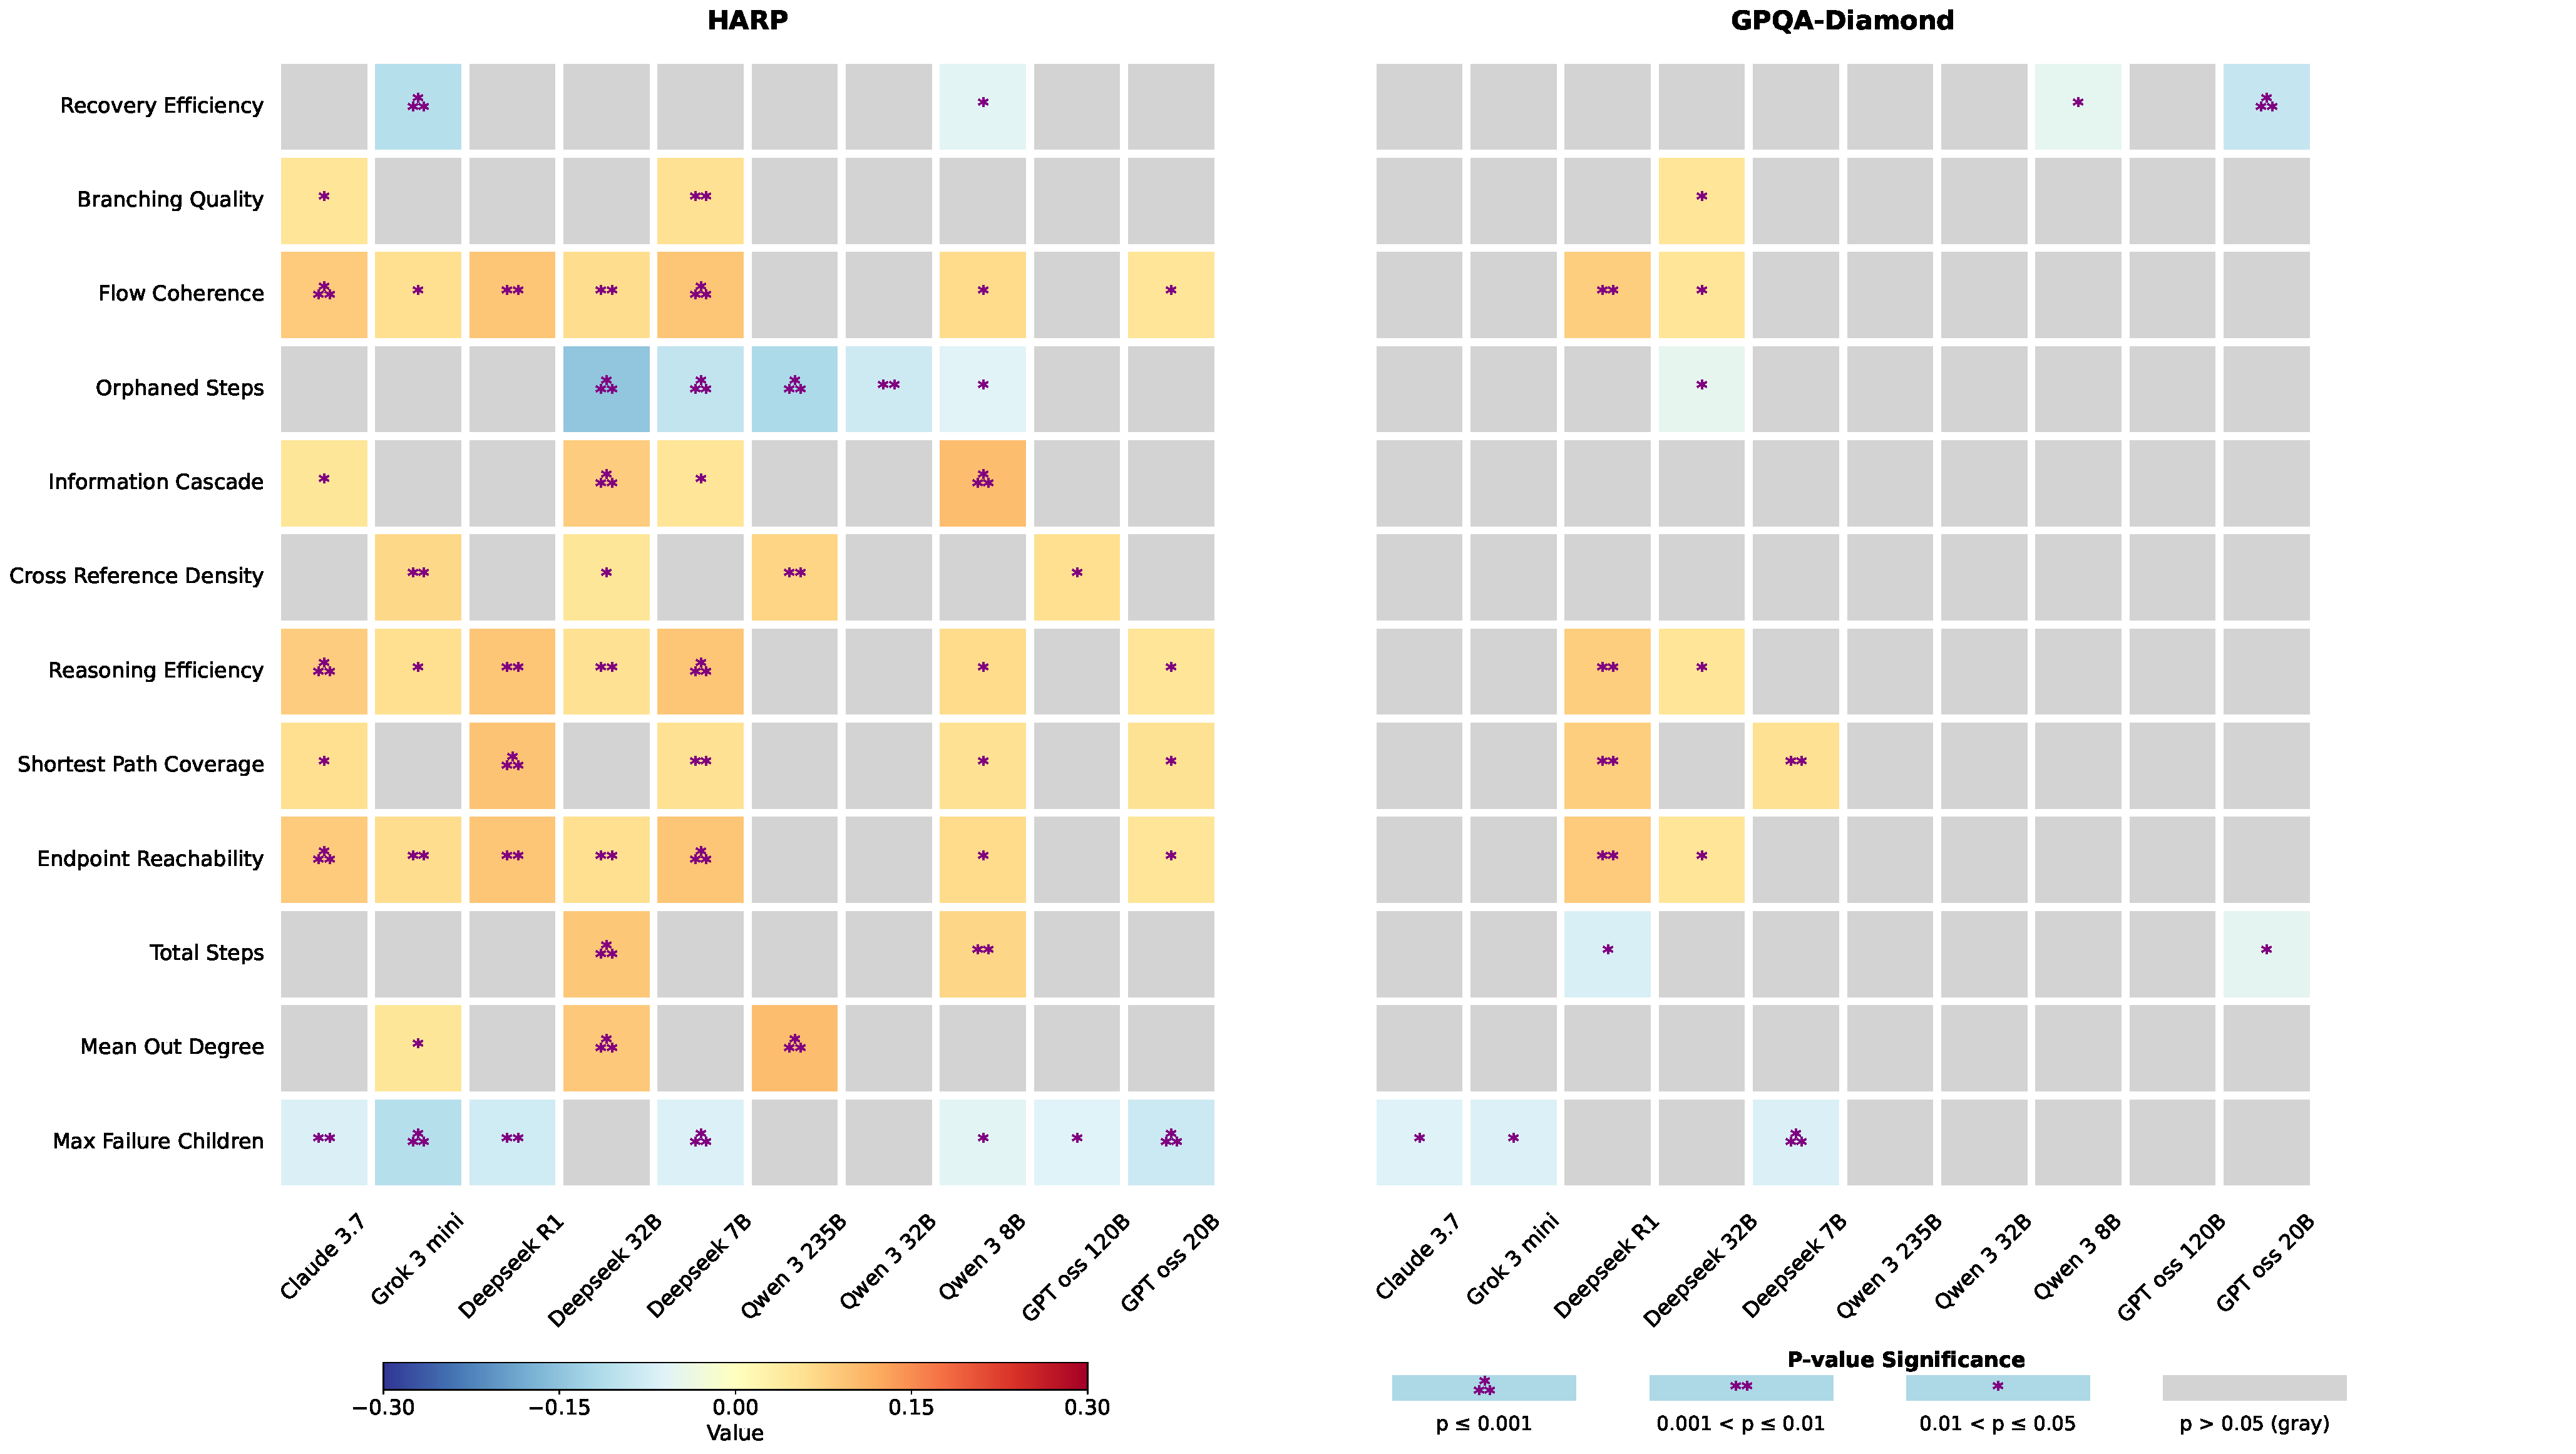
\includegraphics[width=\linewidth]{final_figs/correlation_graphs.pdf}
    \caption{Correlation results for extra graphical metrics, computed on the full dataset. Again, correlations are shown with a color scale; non-significant cells (\(p>0.05\)) are grayed out, and * denotes statistical significance. Overall, these metrics are weaker than \fsf, with significant correlations appearing primarily in mathematical reasoning. We color * white or purple for visualization only. }
    \label{fig:correlation_graphs}
\end{figure}

\section{Intervention Details}\label{append-intervention}

\subsection{Test-time Selection}

Beyond the test-time selection results in Figure~\ref{fig:pass_1_aime} (AIME-2025), we repeat the experiment on HARP. Specifically, we sample 180 questions (60 each from Levels 4, 5, and 6), disjoint from those used in our correlation analyses. For each question, we generate 64 CoTs and select the top-1 candidate under each metric.

The results in Figure~\ref{fig:pass_1_harp} show improvements for Claude 3.7, Grok 3 mini, and Deepseek R1 that mirror Figure~\ref{fig:pass_1_aime}. By contrast, Qwen exhibits anomalous behavior: selecting the generation with the smallest \length or the smallest \rr drives accuracy to \(0\). We hypothesize that this stems from train–evaluation contamination: these hard math problems (from past U.S. math olympiad contests) are likely included in Qwen’s training (Reinforcement Learning from Verifiable Reward), leading to atypical selection dynamics. On contamination-minimized datasets (AIME 2025 and GPQA-Diamond), Qwen follows the same trend as the other models. Accordingly, we present the clean test-time selection results on these two datasets in the main paper, with AIME 2025 providing the most contamination-free evaluation.


\begin{figure}
    \centering
    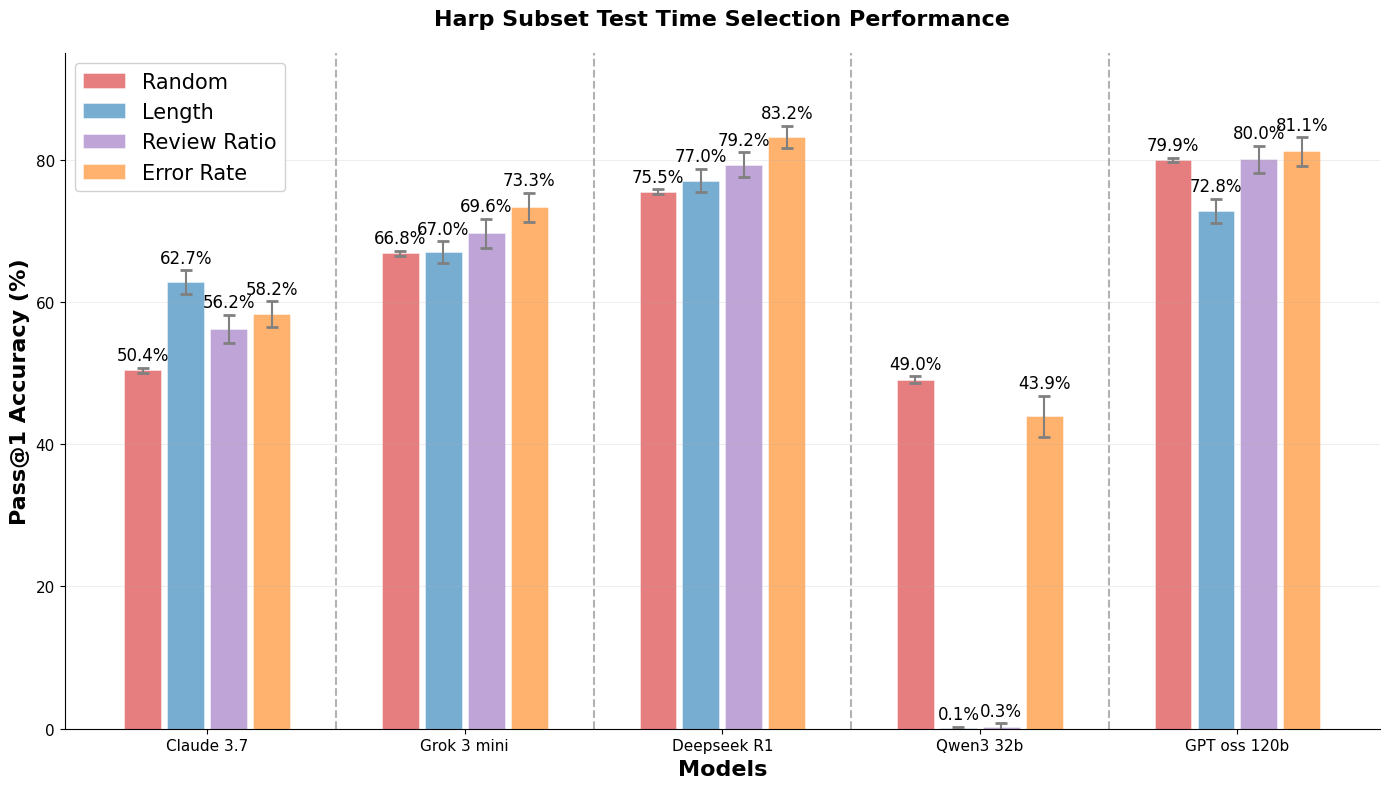
\includegraphics[width=0.7\linewidth]{fig_tmp/pass_1/pass_1_harp.png}
    % \includegraphics[width=0.45\linewidth]{fig_tmp/pass_1/harp_test_time_qwen_judge.png}
    \caption{Pass@1 with test-time selection by \length, \rr, and \fsf on HARP subset. Error bars show bootstrap standard deviations. Qwen exhibits weird results, likely because most evaluation questions appear in its RL training data. Excluding Qwen, \fsf-based selection consistently identifies higher-quality generations at test time.}
    \label{fig:pass_1_harp}
\end{figure}

\subsection{Controlled Editing of the CoT}

In the intervention experiment, we need to identify where the failed branch begins and ends to remove it completely. We break it into several tasks, when Claude model extract the reasoning graph, we further ask it to (i) list each reasoning step and output the first 20 words of that step, and (ii) for each failed attempt step, mark the index at which the failed branch starts. (i) helps us build a mapping between the step in the graph to the sentences and paragraphs in the reasoning chain. We then align the returned quotations to the original CoT using n-gram matching (to tolerate minor misquotations). (ii) helps us to identify where to remove. We perform all of them together in one prompt, with the following prompt appended after the graph-extraction prompt.

The prompt used (to be appended after the graph-extraction prompt) is:


\fbox{\parbox{0.9\textwidth}{
Additionally, provide a separate list with the exact format below:

List of nodes with first 20 words:

1. node id: "exact first 20 words of this reasoning step"

2. node id: "exact first 20 words of this reasoning step"

3. node id: "exact first 20 words of this reasoning step"

...
\\
\\
Requirements:

- Use numbered list format: "number. node id: "quoted text""

- Each entry must be on a single line

- Preserve exact formatting, punctuation, line breaks, and special characters from the original reasoning trace

- Use double quotes around the 20-word excerpts; the 20-word should be exactly the first 20 words of the reasoning step.

- Node IDs should match exactly with the DOT code node names

- This list should enable precise string matching back to the original reasoning trace
\\
\\
Example format:

1. problem statement: "Solve the following math problem efficiently and clearly. Please reason step by step, and put your final answer within \$\textbackslash boxed\{answer\}\$."

2. analysis step: "First, let me understand what we're given. We have a triangle with specific angle measures and need to find the missing side length."

After these, for each failed attempts you have labeled as lightpink, tract the entire reasoning branch, also provide:
\\
\\
Branch Analysis:

1. node id, starts from node id "name", fails to current node id.
\\
\\
The definition: For each failed reasoning attempt (pink node), identify the most recent successful node (blue node) from which this failed path originally diverged, marking that successful node as the branch starting point where alternative reasoning paths split off.
The next reasoning step after the current failed attempt should directly starts again from the node just before this branching starting point.
}}

\section{Further Findings}\label{append:further}

\subsection{Progressiveness and Entropy.}

\paragraph{Progressiveness and Entropy.}
Motivated by recent work \citep{wu2025knowledge}, we evaluate how quickly a model converges to an answer (progressiveness) and how its answer entropy evolves along the CoT. The answer entropy measures how confident the model is with the answer. At multiple prefix truncations within each trace (0\%, 25\%, 50\%, 75\%), we append
\textit{I have thought long enough. Now let me conclude: the final answer is}
to elicit a distribution over answers. We sample 8 continuations per truncation position and estimate confidence via the empirical answer entropy
\[
H_t \;=\; -\sum_{a} \hat{p}_t(a)\,\log \hat{p}_t(a),
\quad\text{where } \hat{p}_t(a) \text{ is the frequency of answer } a \text{ at checkpoint } t.
\]

Compared with accuracy alone, the entropy captures the confidence and directly measures information accumulation. The actual information gain can be extracted with area under the curve, with normalization to $[0, 1]$ for the steps, 
\texttt{Progressiveness}: For reasoning trace $r=\{c_t\}_{t=1}^{T}$:
    \begin{equation}
        \texttt{Progressiveness}(r) = H_0 - \frac{1}{T}\sum_{t=1}^{T}H_t.
    \end{equation}

\paragraph{Findings.} Figure~\ref{fig:truncation_length_diff_2} plots entropy and accuracy as functions of the truncation rate for CoTs on HARP, comparing Deepseek R1 and Qwen 3 8B. The x-axis denotes the truncation rate (fraction of characters removed from the end of the CoT): 0\% = no truncation (original CoT), 95\% = remove the last 95\% of characters. Across models and difficulty levels, entropy declines along the CoT with strikingly similar trajectories, and terminal entropy is low regardless of whether the final answer is correct or incorrect. In other words, models end up confident—even when wrong. Consequently, we do not include progressiveness and answer entropy in our correlation analyses.

% We report the entropy trajectories for Deepseek R1 and Qwen 3 8B in Figure \ref{fig:truncation_length_diff_1}.

In Figure~\ref{fig:truncation_length_diff_2}, for each question we partition CoTs into a \emph{short} half and a \emph{long} half (by length) and report accuracy for each group across truncation rates. Across all difficulty levels, the \emph{short} group attains higher accuracy, reinforcing that shorter CoTs correlate with higher accuracy.




% \begin{figure}[h]
%     \centering
%     \includegraphics[width=0.8\linewidth]{fig_tmp/difficulty_cross.png}
%     \caption{How model difficulty and human labeled difficulty differs.}
%     \label{fig:difficulty_cross}
% \end{figure}


% \begin{figure}[htb]
%     \centering
%     \includegraphics[width=\linewidth]{fig_tmp/truncation_length_diff_1.png}
%     \caption{Impact of CoT truncation on answer entropy and correctness across difficulty strata. The x-axis is the truncation rate from the end of the CoT (e.g., 0 = no truncation, 0.5 = last half removed). Top: Deepseek R1; Bottom: Qwen 3 8B.}
%     \label{fig:truncation_length_diff_1}
% \end{figure}

\begin{figure}[htb]
    \centering
    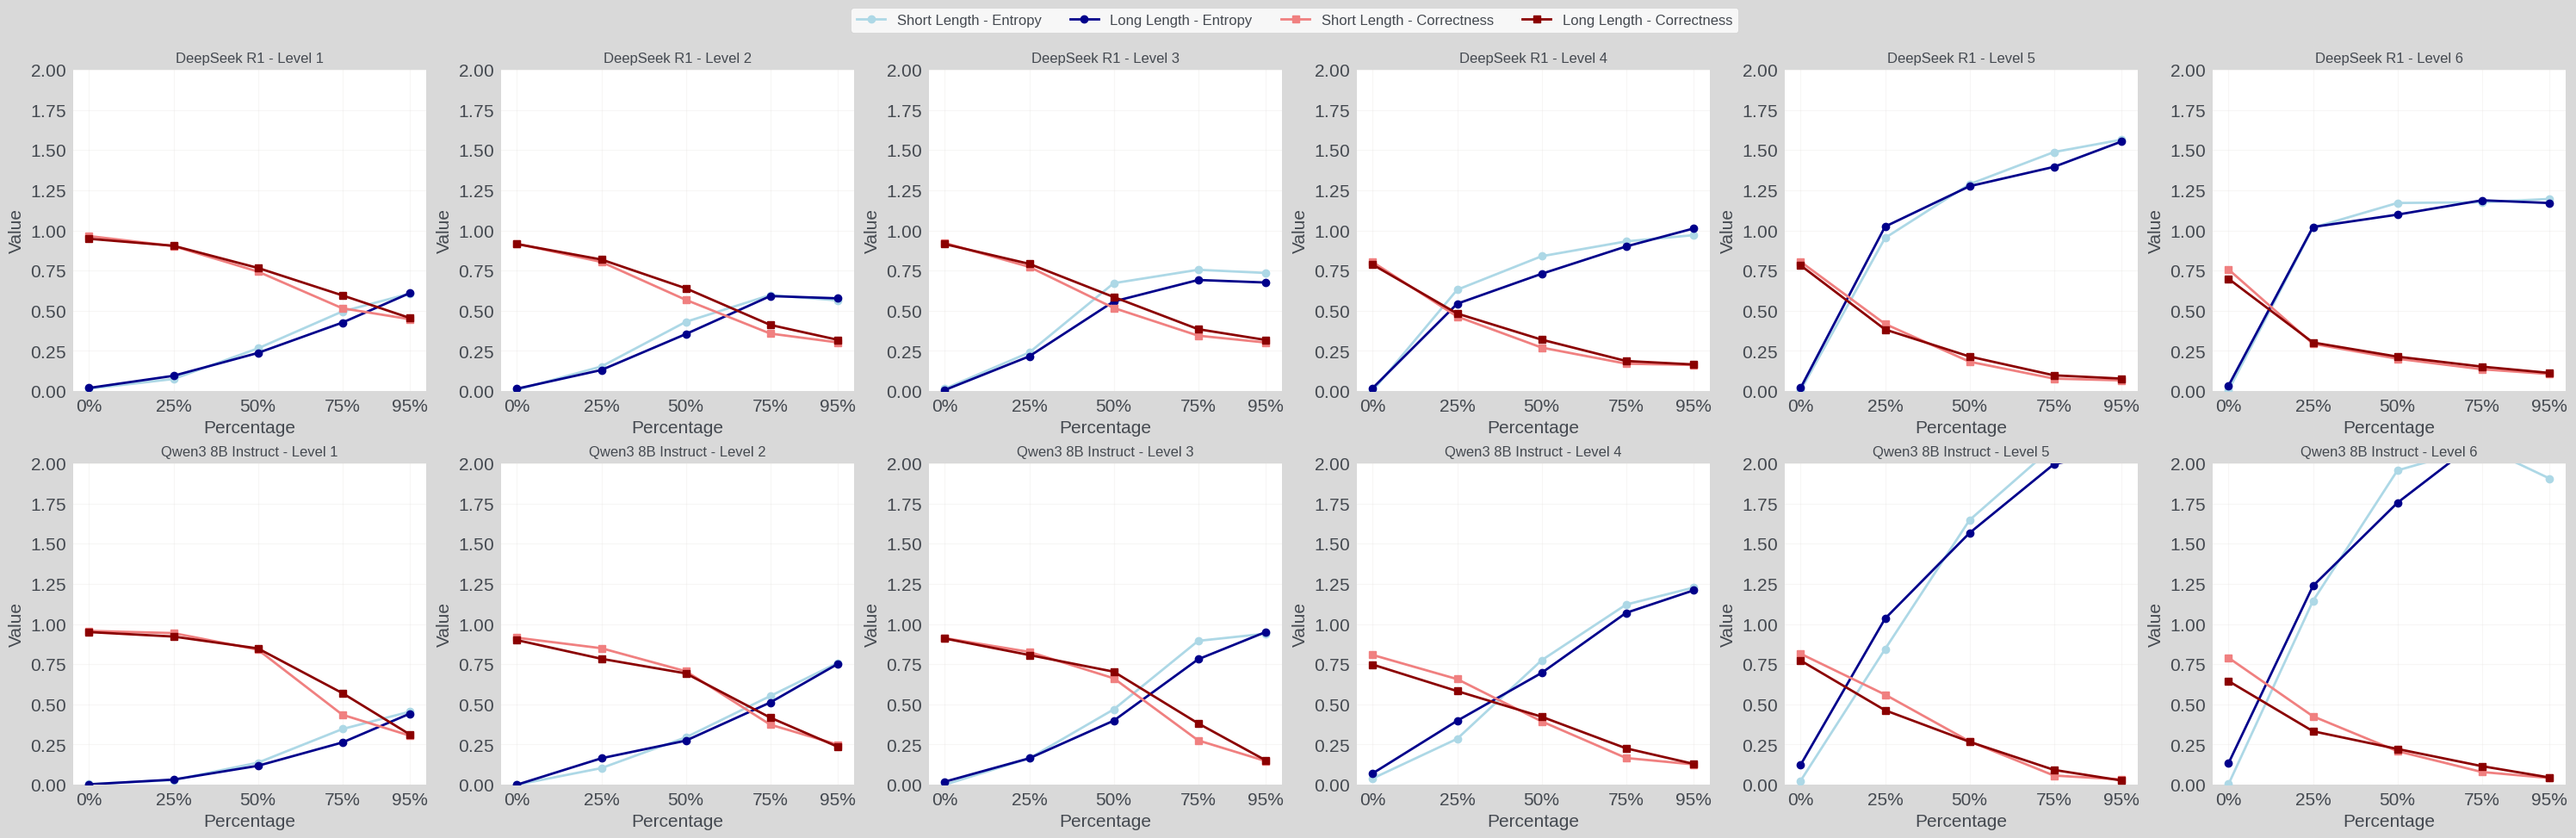
\includegraphics[width=\linewidth]{fig_tmp/truncation_length_diff_2.png}
    \caption{Impact of CoT truncation on answer entropy and correctness across difficulty strata. Within each question, we partition CoTs into \emph{short} and \emph{long} groups to compare length effects. The x-axis reports the truncation rate from the end of the CoT (e.g., 0 = no truncation; 0.5 = last half removed). Top: Deepseek R1; Bottom: Qwen 3 8B.}
    \label{fig:truncation_length_diff_2}
\end{figure}


\subsection{How different models behave?}

Finally, we are also interested in how different models have different behaviors on model level. Thus, we aggregate the average \Length, \rr, and \failedstep for each model, and plot its distribution with model's accuracy. We present the results in Figure \ref{fig:harp_models_distribution}.

We do not observe a correlation pattern that holds uniformly across models. The clearest cross-model signal is \fsf—especially on GPQA-Diamond—where models with lower \fsf tend to achieve higher accuracy. The absence of universal trends is intuitive: output style strongly affects these metrics, particularly \length and \rr. Some models “over-verify” \citep{chen2024not}, inflating \length and \rr without necessarily lowering accuracy if the problem is ultimately solved. This further supports our decision not to pool CoTs across models. Instead, we take a more debiased analysis: we estimate correlations \emph{within} each model and then look for patterns that replicate \emph{across} models.

\begin{figure}[tb]
    \centering
    \text{(a) HARP}
    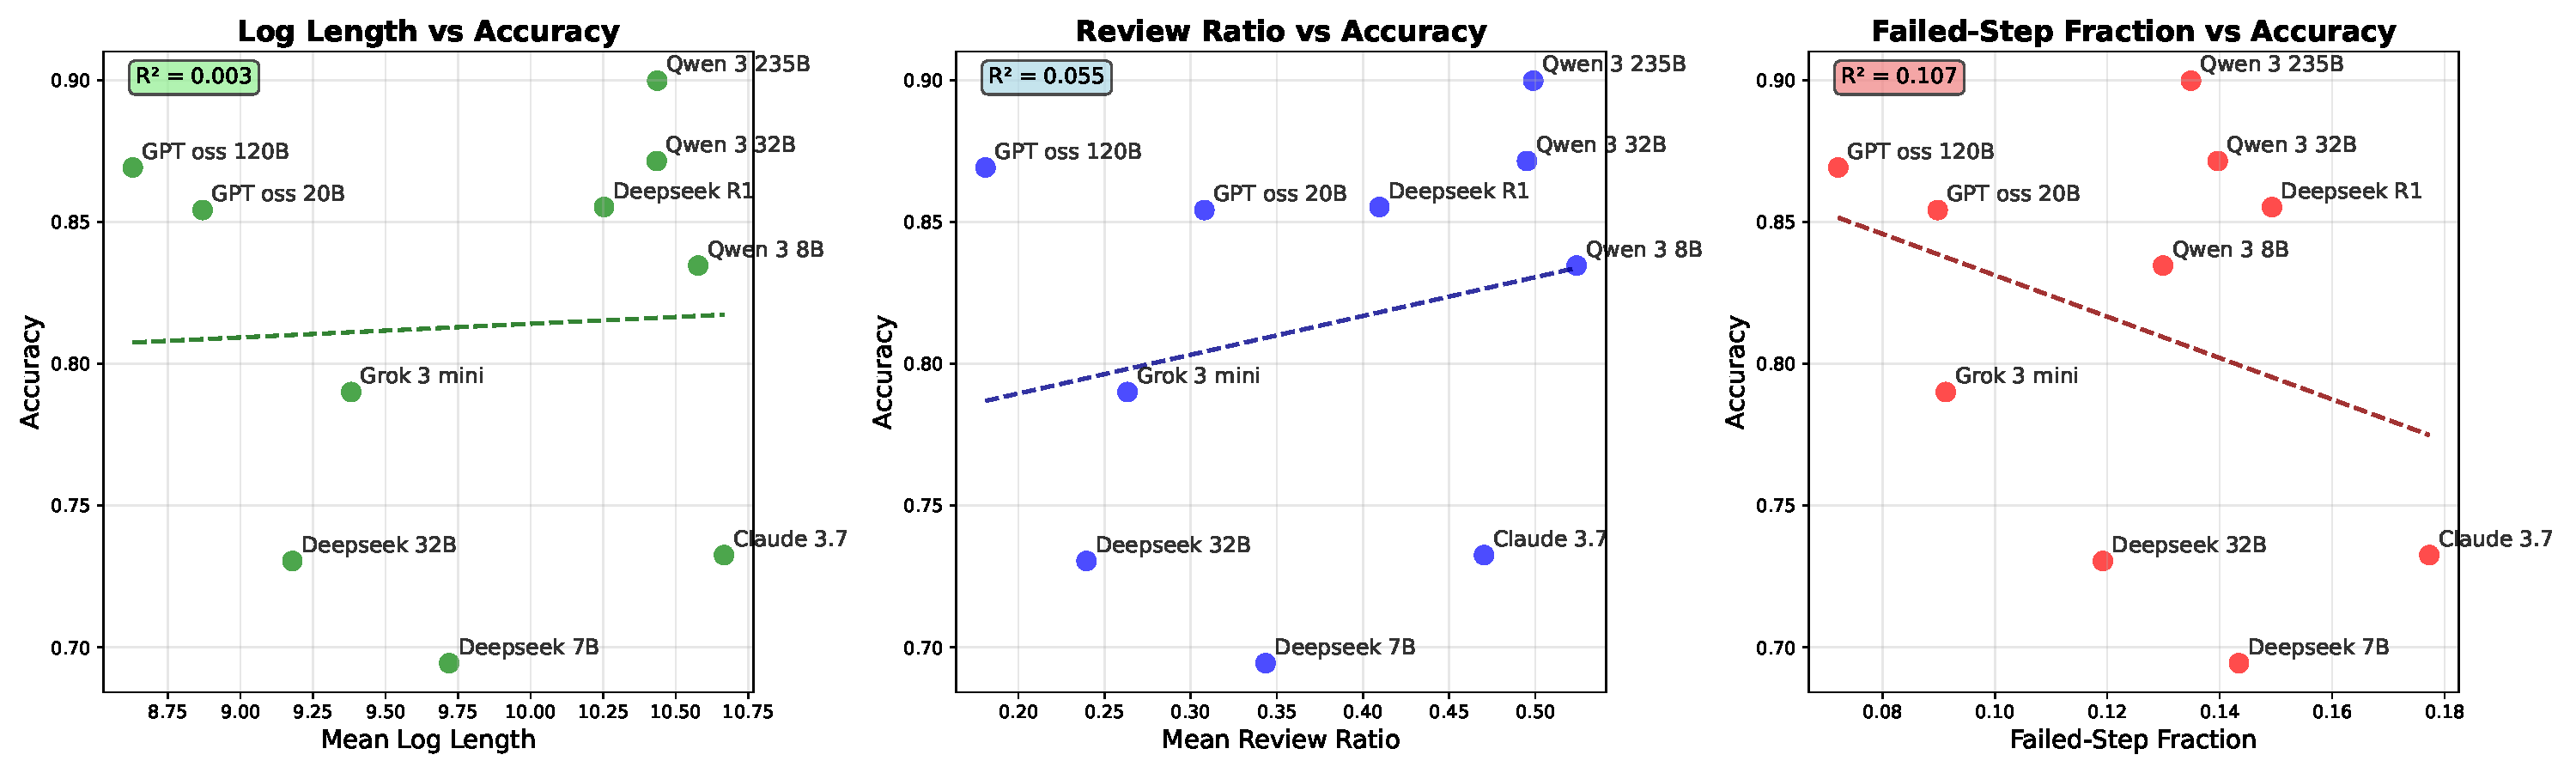
\includegraphics[width=1\linewidth]{final_figs/harp_models_distribution.pdf}
    % \vspace{10pt}
    \text{(b) GPQA-Diamond}
    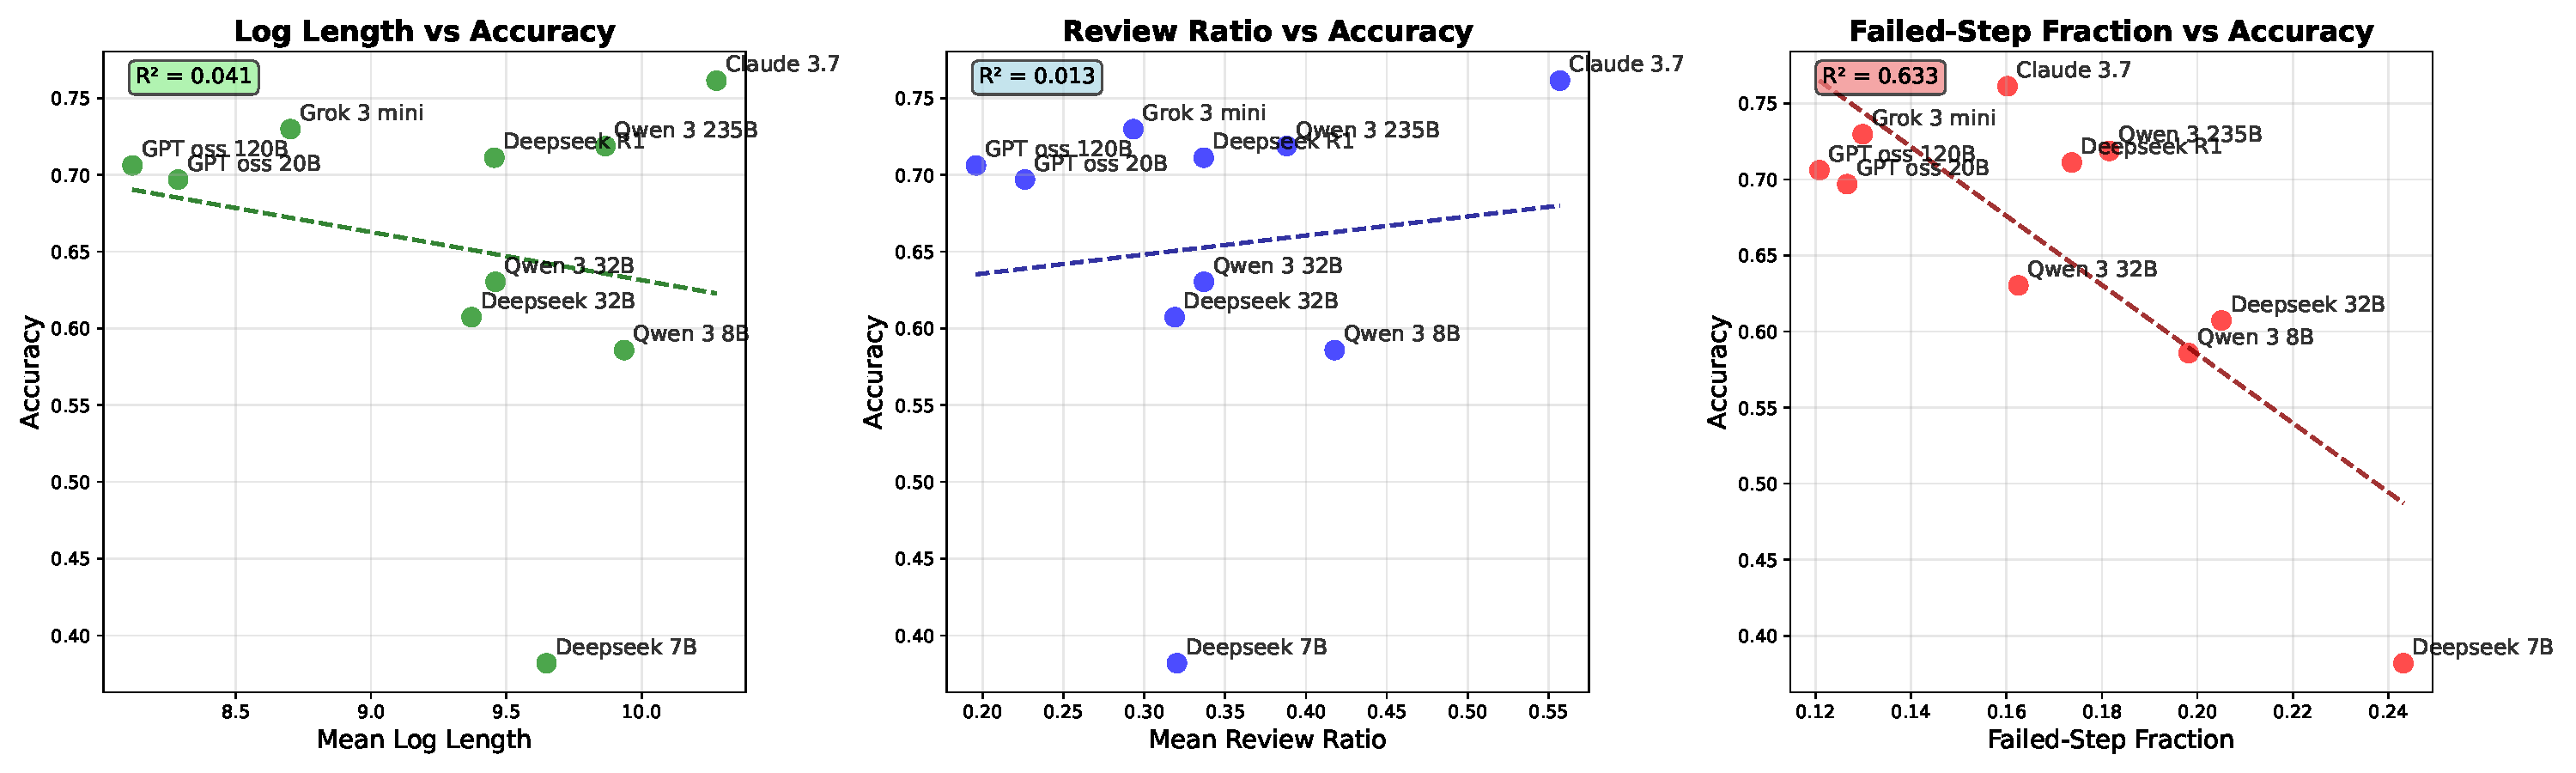
\includegraphics[width=1\linewidth]{final_figs/gpqa_models_distribution.pdf}
    \caption{Model-level relationship between accuracy and average behavior (\length, \rr, \fsf). Top: HARP; Bottom: GPQA-Diamond. Overall, we do not observe consistent cross-model patterns: these features are largely model-specific. Though \fsf shows some correlation across models, especially for GPQA-Diamond.}
    \label{fig:harp_models_distribution}
\end{figure}

% \begin{figure}
%     \centering
%     \includegraphics[width=0.45\linewidth]{fig_tmp/pass_1/aime_test_time_claude.png}
%     \includegraphics[width=0.45\linewidth]{fig_tmp/pass_1/aime_test_time_grok.png}
%     \includegraphics[width=0.45\linewidth]{fig_tmp/pass_1/aime_test_time_deepseek_r1.png}
%     \includegraphics[width=0.45\linewidth]{fig_tmp/pass_1/aime_test_time_qwen3.png}
%     \caption{Using different metrics as test-time selection metric, to improve the generation quality. Evaluation for all pass@k. Select with figure? AIME 2025.}
%     \label{fig:test_time}
% \end{figure}

